%CHAPTER
\chapter{Formát PDF}
Formát \textbf{PDF} (\textbf{P}ortable \textbf{D}ocument \textbf{F}ormat) je souborový formát vyvinutý společností Adobe v~roce 1992. Formát PDF byl vyvinut za účelem konzistentní prezentace dokumentů na různých platformách. Díky konzistenci lze dosáhnout toho, že soubor PDF vytvořený a uložený v~systému Windows bude zobrazen totožně na systémech Mac, na všech distribucích Linuxu nezávisle na použitém prohlížeči PDF (Adobe Reader, Foxit a další).
\par 
V~souboru PDF lze uchovávat velice širokou škálu dat, včetně formátovaného textu, vektorové grafiky a rastrových obrazů, nebo například informace o~rozložení, velikosti a tvaru stránky. Informace definující umístění jednotlivých položek (jsou zde zahrnuty i editovací objekty pro formuláře) na stránce jsou zde uloženy též. Do dokumentu lze ukládat i metadata. Metadata jsou informace uložené v~hlavičce souboru a lze do nich uložit název dokumentu, autora dokumentu, předmět a klíčová slova. Je zde možnost uložit heslo, aby byl dokument přístupný pouze autorizovaným uživatelům. Všechny tyto informace jsou uloženy ve standardním formátu \cite{PDFTechTerms, PDFWhatIs}.

%SECTION
\section{Objekty}
PDF objekty jsou základním stavebním kamenem pro uchovávání dat v~dokumentu. Množinou PDF objektů lze reprezentovat bitmapové a vektorové objekty, barevné prostory, text, fonty aj. \cite{PDFExplained}.
%SUBSECTION
\subsection{Základní objekty}
V~PDF můžeme najít celkem pět základních objektů:
	\begin{itemize}
		\item \verb|Celá a reálná čísla| --  Přesnost a rozsah celých a reálných čísel je definován jednotlivými implementacemi PDF. V~některých implementacích platí pravidlo, které přetypuje celé číslo na reálné po přesáhnutí předem daného rozsahu.
		\item \verb|Řetězce| -- Řetězec je reprezentován jako množina po sobě jdoucích bytů vepsaných mezi jednoduché závorky. Jako příklad lze uvést: \textit{(Hello, World!)}. Pro zobrazení zpětného lomítka a jednoduchých závorek je potřeba před tyto znaky přidat zpětné lomítko pro jejich správné zobrazení v~dokumentu. V~tabulce \ref{tab:table_escaped} lze vidět využití zpětného lomítka pro zobrazení odřádkovacích znaků:
			\begin{table}[h!]
			\centering
			\begin{tabular}{|l|l|} 
			\hline
			\textbf{Sekvence znaků}    & \textbf{Význam}                \\ 
			\hline
			\textit{\textbackslash{}n} & \textit{Line feed (LF)}        \\ 
			\hline
			\textit{\textbackslash{}r} & \textit{Carriage return (CR)}  \\ 
			\hline
			\textit{\textbackslash{}t} & \textit{Tab}                   \\ 
			\hline
			\textit{\textbackslash{}b} & \textit{Backspace}                      \\
			\hline
			\end{tabular}
			\caption{Odřádkovací sekvence znaků}
			\label{tab:table_escaped}
			\end{table}
		\newline Řetězce můžou být reprezentovány i jako sekvence hexadecimálních čísel vložených mezi znaky \verb|<| a \verb|>|. 
		\newline Jako příklad lze uvést: \textit{<4F6EFF00> -- 0x4F, 0x6E, 0xFF, 0x00}.

		\item \verb|Jména| -- Jméno je reprezentováno jako sloučení lomítka a řetězce (př. \textit{/Jmeno}). Za jméno se pokládá i zpětné lomítko bez řetězce. Pokud bychom potřebovali nadefinovat v~dokumentu jméno, jenž bude obsahovat mezery, musíme do řetězce přidat i sekvenci znaků \textbf{\#20} (v~tabulce ASCII je hexadecimální hodnota dvacet vyjádřena jako prázdný znak). U~jmen se rozlišují velká a malá písmena, proto \textit{/Jmeno} a \textit{/jmeno} jsou dvě různá jména. Jeho využití v~PDF je prosté, slouží jako klíče ve slovnících a pro definice složitějších (vícehodnotových) objektů.
		\item \verb|Boolean (pravdivostní) hodnoty| -- Logické hodnoty \textbf{true}/\textbf{false} a vyskytuje se v~jednotlivých záznamech ve slovníku jako příznak.
		\item \verb|Hodnota null| -- Nabývá hodnot \textit{f} (free) nebo \textit{n} (use) a vyjadřuje, zda je objekt vyobrazen v~dokumentu.
	\end{itemize}
%SUBSECTION
\subsection{Složené objekty}	
Složený objekt je takový objekt, který obsahuje seřazenou/neseřazenou množinu základních objektů i množinu složených objektů.
	\begin{itemize}
		\item \verb|Pole| -- Pole je v~PDF reprezentováno jako seřazená množina základních i složených PDF objektů (v~poli může být uložen například i slovník nebo pole) nezávisle na typech (v~poli lze uchovávat například řetězec a číslo zároveň). Hodnoty pole jsou vloženy mezi znaky \verb|[| a \verb|]|.
		\item \verb|Slovníky| -- Slovník se skládá z~množiny dvou prvků: klíče a hodnoty, pomocí kterých se slovník namapuje. Klíč je reprezentován pomocí \textbf{jména}, zatímco hodnota může být kterýkoliv PDF objekt, povoleny jsou i slovníky nebo pole. Slovníky jsou uloženy mezi znaky \verb|<<| a \verb|>>|.
		\item \verb|Datové proudy| -- Datové proudy slouží především pro uložení binárních dat a skoro ve všech případech jsou zkomprimovány různými kombinacemi algoritmů, které jsou popsány v~kapitole \ref{sec:komprese}, proto datové proudy musí být zároveň i nepřímým odkazem (odkaz na objekt obsahující data). Datové proudy se skládají ze slovníků a části binárních dat. Slovník je využit pro ukládání parametrů binárních dat, jako například délka binárních dat aj.
	\end{itemize}
%SUBSECTION
\subsection{Linkovací objekty}
PDF objekty můžou být různě velké. Pokud je objekt až příliš veliký, pak jsou v~kódu dokumentu využity nepřímé odkazy. Na obrázku \ref{fig:indirect_reference} si lze všimnout využití nepřímých odkazů ve slovníku. 
	\begin{figure}[h!]
	\centering
	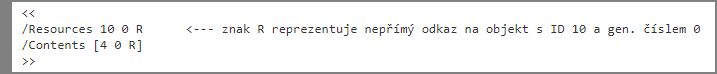
\includegraphics[width=15cm]{img/pdf_indirect_reference}
	\caption{Ukázka nepřímého odkazu}
	\label{fig:indirect_reference}
	\end{figure}

%SECTION
\section{Komprese dat v~PDF}
\label{sec:komprese}
Soubory PDF mohou být poměrně kompaktní, o~mnoho menší než ekvivalentní soubory vytvořené v~\textbf{PostScriptu} (programovací jazyk určený ke grafickému popisu tisknutelných dokumentů vyvinutý v~roce 1985 firmou Adobe Systems Incorporated). Tato vlastnost je dosažena nejen lepší strukturou dat, ale i díky kompresním algoritmům, které jsou efektivní. Typ komprese dat souboru PDF lze zjistit pomocí textového editoru, který dokáže zpracovat binární data, vyhledáním klíčového slova \textbf{/Filter}. Níže jsou popsány kompresní algoritmy využívané v~PDF \cite{PDFPrepressure}.
\begin{itemize}
	\item \verb|CCITT G3/G4| -- Algoritmus je bezeztrátový a využívá se pro vykreslení černobílých obrázků.
	\item \verb|JPEG| -- JPEG algoritmus může být jak ztrátový, tak i bezeztrátový. V~Acrobatu se využívá pouze ztrátový s~pěti stupni komprese. Využívá se pro barevné a šedotónové obrázky.
	\item \verb|JPEG2000| -- Rychlejší algoritmus na bázi JPEGu. Víceméně se nepoužívá, jelikož není kompatibilní se staršími systémy a má vysoké nároky na procesor.
	\item \verb|Flate| -- Bezeztrátový algoritmus, vychází z~kompresních algoritmů LZ77 a Huffmanova kódování.
	\item \verb|JBIG2| -- Alternativní k~CCITT. V~Dnešní době se nevyužívá z~důvodu pomalejší komprese než je u~jeho protějšku.
	\item \verb|LZW| -- Komprimací LZW algoritmem lze dosáhnout až o~polovinu menší velikosti díky komprimaci veškerého textu a operátorů v~souboru.
	\item \verb|RLE| -- Bezeztrátový algoritmus pro vykreslování černobílých obrázků. Nahrazen efektivnějším algoritmem CCITT.
\end{itemize}

%SECTION
\section{Vnitřní struktura PDF}
\label{subsec:vnitrni_struktura}
Vnitřní reprezentace souboru PDF je rozdělena na sekce, které jsou znázorněny na obrázku \ref{fig:pdf_internal_structure}.

\begin{figure}[h!]
\centering
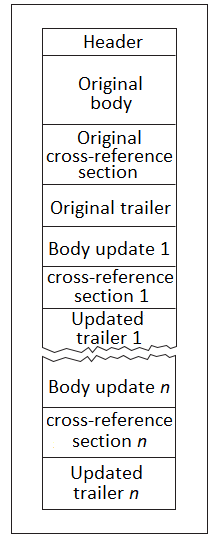
\includegraphics[width=4cm]{img/pdf_internal_structure}
\caption{Interní struktura souboru PDF}
\label{fig:pdf_internal_structure}
\end{figure}

Z~obrázku lze vyčíst, že se zde vyskytují čtyři hlavní sekce: \textit{Header}, \textit{Body}, \textit{Cross-reference} a \textit{Trailer}. Díky jedné z~vlastností formátu PDF se při úpravě souboru staré sekce neodstraní, místo toho se pouze na jeho konci vytvoří nové sekce \cite{PDFInfoSec}.
\begin{itemize}
	\item \verb|Header| -- Hlavička souboru je uložena na první řádce, obsahující primárně použitou verzi PDF.
	\begin{figure}[h!]
	\centering
	
\includegraphics[width=15cm]{img/pdf_hlavicka}
	\caption{Ukázka hlavičky}
	\label{fig:pdf_header}
	\end{figure}
	
	\item \verb|Body| -- V~těle dokumentu jsou uložena veškerá data objektů reprezentující celý dokument. Objekty jsou referencovány v~tabulce Cross-reference z~důvodu rozprostření částí dat patřících k~danému objektu po celé sekci.Pokud se v~dokumentu vyskytuje jeden obrázek/zvukový záznam vícekrát než jednou, tak se poté všechny objekty reprezentující obrázky odkazují na jednu množinu dat \cite{PDFAdobe}.
	\begin{figure}[h!]
	\centering
	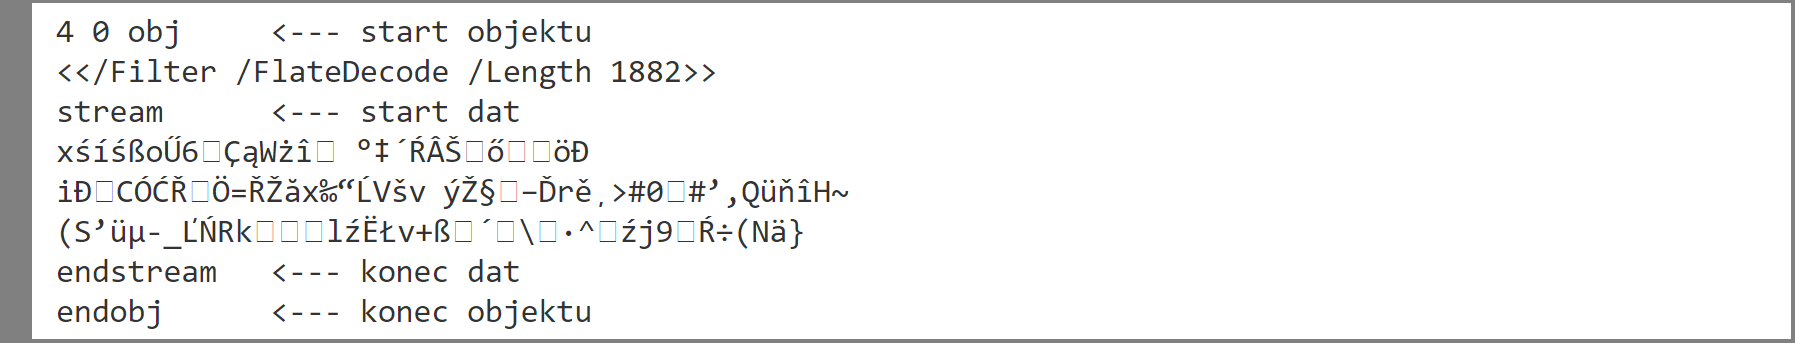
\includegraphics[width=15cm]{img/pdf_body}
	\caption{Ukázka dat objektu}
	\label{fig:pdf_body}
	\end{figure}

	\item \verb|Cross-reference table| -- Jinak nazývána \textbf{xref} je tabulka obsahující reference na veškeré objekty uložené v~těle a v~kódu začíná řetězcem \textit{xref}. Reference uložená v~tabulce je reprezentována na dvou řádcích pomocí řetězce a skládá se z~pěti částí o~celkové velikosti dvacet bytů včetně oddělovačů \textit{CRLF} (Windows), \textit{CR} (Mac OS), \textit{LF} (Unix, Linux):
	\begin{itemize}
		\item \textit{Číslo objektu} -- Jednoznačný číselný identifikátor objektu.
		\item \textit{Počet subobjektů} -- Počet částí daného objektu vyskytujícího se v~dokumentu.
		\item \textit{Začátek objektu} -- Tvoří většinu řetězce (prvních deset bytů) a určuje offset od začátku dokumentu PDF až po začátek daného objektu.
		\item \textit{Generační číslo objektu} -- Vyjadřuje, jak často byl objekt vymazán při úpravě dokumentu. 
		\item \textit{Identifikátor využití} -- Nabývá hodnot \textit{f} (free) nebo \textit{n} (use) a vyjadřuje, zda je objekt vyobrazen v~dokumentu.
	\end{itemize}
	\begin{figure}[h!]
	\centering
	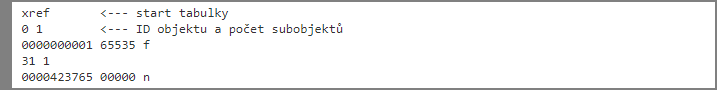
\includegraphics[width=15cm]{img/pdf_xref}
	\caption{Ukázka jednoduché xref tabulky}
	\label{fig:pdf_xref}
	\end{figure}

	\item \verb|Trailer| --  Trailer je seznam informací, ze kterých lze snadno zjistit například velikost nebo umístění xref tabulky. Trailer může obsahovat tyto elementy:
	\begin{itemize}
		\item \textit{Size} -- Udává počet objektů referencovaných v~xref tabulce. 
		\item \textit{Prev} -- Offset od začátku dokumentu k~předchozí xref tabulce.
		\item \textit{Root} -- Odkazuje na objekt obsahující informace ohledně katalogu xref tabulek.
		\item \textit{Encrypt} -- Specifikuje komprimační algoritmus použitý pro daný dokument.
		\item \textit{Info} -- Obsahuje dodatečné informace ohledně katalogu xref tabulek.
		\item \textit{ID} -- 2-bytový identifikátor dokumentu PDF.
		\item \textit{XrefStm} -- Offset od začátku dokumentu až k~dekódovanému xref streamu. Využívá se pouze u~hybridně-referencovaných (v~raw kódu jsou využity přímé i nepřímé odkazy) souborů za předpokladu že hledaný objekt není nalezen v~xref tabulce (před tím, než se volá element \textit{Prev}). 
	\end{itemize}
	\begin{figure}[h!]
	\centering
	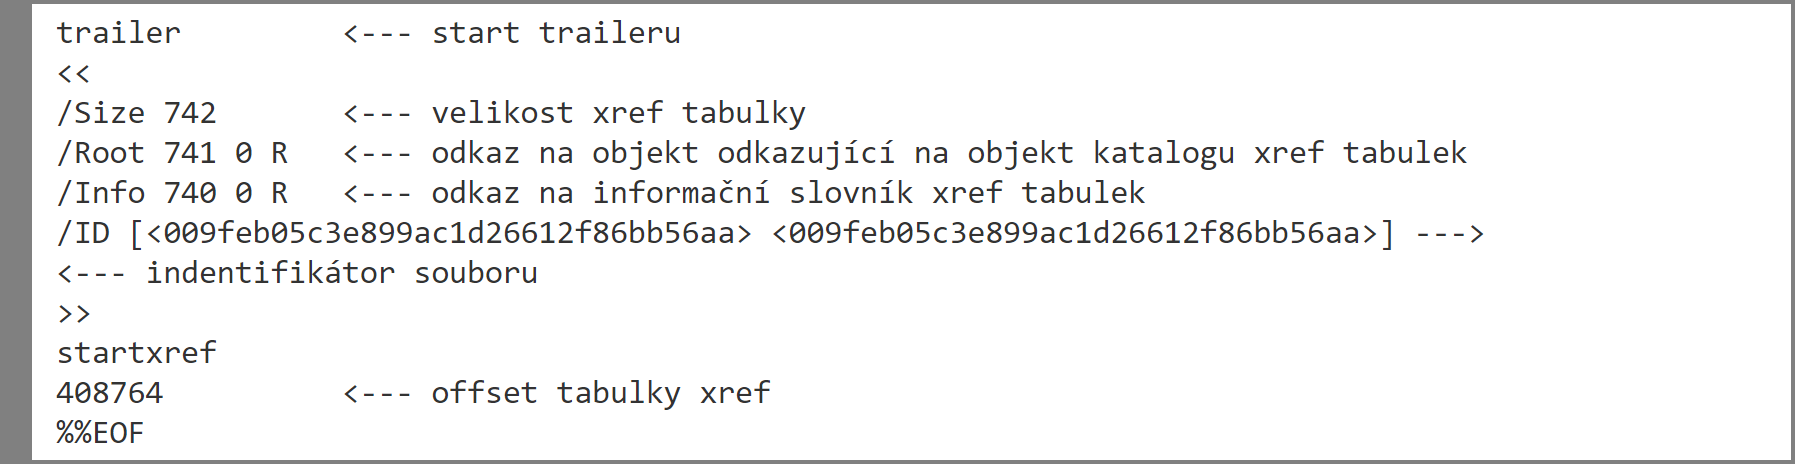
\includegraphics[width=15cm]{img/pdf_trailer}
	\caption{Ukázka traileru}
	\label{fig:pdf_trailer}
	\end{figure}
\end{itemize}
%SECTION
\section{PDF formuláře}
Pod pojmem formulář si lze představit dokumenty, které od svých uživatelů vyžadují vyplnění určitých údajů. Mezi nejznámější dokumenty lze například uvést daňová přiznání, oznamovací tiskopisy a dotazníky. Ruční vyplňování i jejich následné zpracování bývá obvykle pracné a zdlouhavé, proto je v~dnešní době výhodnější využívat interaktivní elektronické formuláře. Základní výhoda těchto formulářů spočívá ve zrychlené komunikaci mezi objekty a subjekty. Díky elektronické podobě dochází k~úspoře financí. Běžný občas přijde nejčastěji do styku s~přihlašovacími formuláři a různými dotazníky, které jsou ve formátu HTML. Nevýhoda těchto formulářů je v~jejich závislosti na internetovém připojení. 
\par
Proto firma Adobe přišla se svým řešením, interaktivním formulářem PDF, který lze vyplňovat kdekoliv nezávisle na internetovém připojení. Mezi další výhody formulářů PDF patří elektronický podpis (lze s~ním potvrzovat smlouvy z~domova), zabezpečení (dokument se otevře až po zadání správného hesla, neautorizovaným uživatelům je přístup zamítnut) aj. Tyto formuláře obsahují stejné interaktivní prvky jako mají formuláře HTML, viz kapitola \ref{subsec:zakladni_prvky}. Pro generování formulářů PDF lze využít kterýkoliv programovací jazyk, který podporuje práci se soubory PDF (například \textit{PHP}, \textit{Java}), produkty firmy Adobe (například \textit{Adobe Acrobat}) nebo lze použít i nekomerční aplikace typu \textit{TeX} nebo \textit{pdfmarks}.
\par
Tvorba formulářů je jedna věc, druhá věc je jejich zpracování (získání dat vyplněných od uživatele). Mezi nejznámější nástroje pro zpracování vyplněných dat patří určitě nástroj \textit{FDF Toolkit} od firmy Adobe. Tento nástroj je zcela zdarma a umožňuje vytvářet orientovaná řešení pro zpracování dat v~jazycích \textit{C/C++}, \textit{ActiveX}, \textit{Java} a \textit{Perl}. Jsou-li data odeslána v~HTML, lze k~jejich zpracování využít nástroje určené pro formáty \textit{CGI}, \textit{PHP} aj. \cite{PDFForm}.
%SUBSECTION
\subsection{Základní prvky} \label{subsec:zakladni_prvky}
Jednotlivé formulářové prvky mohou mít přiřazeny nejrůznější atributy a jsou reprezentovány jako PDF objekty. Tyto atributy lze rozdělit do následujících skupin: \textbf{Vzhled} (definovaný vzhled prvku), \textbf{Akce} (po kliknutí na prvek se provede daná akce), \textbf{Formát} (typ fontu textu aj.), \textbf{Ověřování dat} (akceptovatelný formát vstupu) a \textbf{Výpočty} (matematické operace použité při práci se vstupy z~jiných prvků) \cite{PDFFormElements}. 
\par
Ve formuláři se může vyskytovat až sedm různých prvků viz obrázek \ref{fig:form_elements}:
	\begin{figure}[h!]
	\centering
	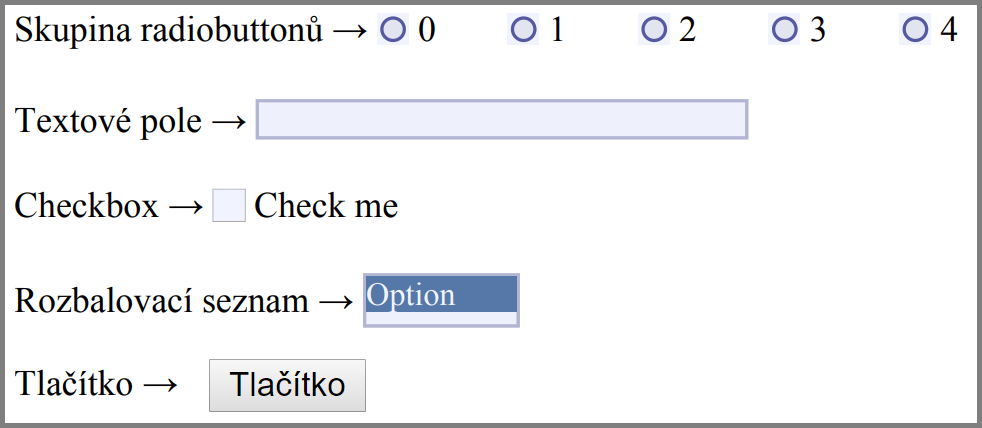
\includegraphics[width=9cm]{img/pdf_form_elements}
	\caption{Základní prvky vyskytující se v~PDF}
	\label{fig:form_elements}
	\end{figure}
	\begin{itemize}
	\item \verb|Textové pole| -- Slouží k~vyplnění textu. Jako příklad lze uvést například klasický přihlašovací formulář, který obsahuje dvě textové pole, jedno pro zadání uživatelského jména a druhé (upravené, místo textu se zobrazují pouze speciální znaky pro zakrytí zadaného textu)  pro zadání hesla. Při vytváření lze předvyplnit toto pole výchozím textem, lze omezit maximální počet znaků vkládaných do pole a jejich formát. Pole může být uzamčeno a může sloužit i jako informační položka.
	\item \verb|Tlačítko| -- Účel tohoto prvku je spouštění zvolených akcí, které se po kliknutí na tlačítko mají provést, tudíž se označují jako hlavní řídící prvek každého formuláře. Tlačítko se skládá převážně z~ikonky a textu, případně mu může být nastaven externí obrázek.
	\item \verb|Seznam| -- Zobrazuje seznam položek, ze kterého lze současně označit jednu nebo více položek (s~využitím klávesy \textit{Shift} nebo \textit{Ctrl}). Pro seznamy lze nastavit filtry, které budou seznam třídit podle předem daných parametrů a zobrazí položky na základě těchto filtrů.
	\item \verb|Kombinované pole| -- Kombinované pole je ve své podstatě seznam prvků, ale liší se ve výběru položek. V~kombinovaném poli lze vybrat pouze jeden aktivní prvek, ostatní budou zakázány. Platí zde pravidla s~tříděním prvků podle filtrů.
	\item \verb|Přepínací tlačítka| -- Je seznam tlačítek, ve kterém uživatel vybírá pouze jednu z~nabízených hodnot.
	\item \verb|Zaškrtávací pole| -- Jedná se o~indikační prvek umožňující současný výběr více položek.
	\item \verb|Podpis| -- Pomocí tohoto prvku lze do dokumentu vložit elektronický podpis.
	\end{itemize}